% 绳的法向压力
% 法向压力|张力|线压强

\pentry{定积分\upref{DefInt}}

我们知道当一根质量忽略不计的绳子紧绷时, 如果它不受任何法相的力(即垂直于绳的力), 它将保持一条直线. 如果绳的一部分存在弯曲, 则说明该部分受法向力. 如\autoref{RopeFP_fig1}, 水平放置的绳子的张力%未完成: 什么时张力
为 $T$, 经过半径为 $R$ 的滑轮后弯曲了 $\theta$ 角. 由于我们假设滑轮与绳之间无摩擦\footnote{等效地, 也可以假设滑轮可以无摩擦滚动}, 经过滑轮后绳的张力仍然为 $T$.
\begin{figure}[ht]
\centering
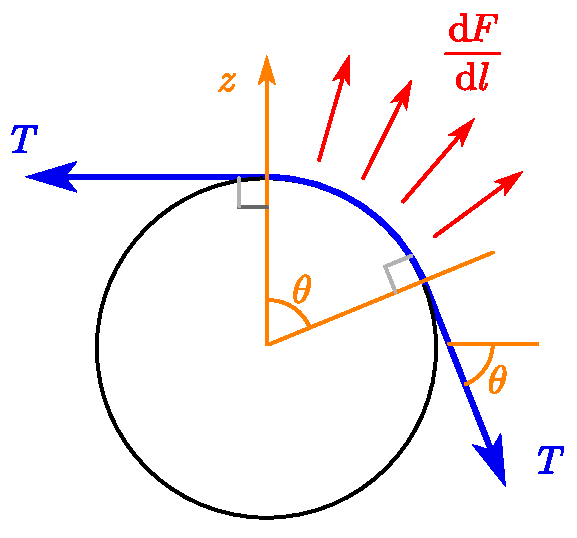
\includegraphics[width=7cm]{./figures/RopeFP_1.pdf}
\caption{滑轮对绳的线压强} \label{RopeFP_fig1}
\end{figure}

显然, 绳弯曲是由于在于滑轮接触的部分处处都受到法向的力. 为了描述这种力的大小, 我们取长度为 $\Delta l$ 的一小段绳(弯曲忽略不计), 若它受法向力大小为 $\Delta F$, 就用 $\Delta F/\Delta l$ 来描述法向力的大小. 当 $\Delta l \to 0$, 就记为 $\dv*{F}{l}$, 称为\textbf{线压强}, 是一个标量(压强是单位面积的压力, 线压强是单位长度的压力). 注意力是相互的, 滑轮对绳的压力于绳对滑轮的压力处处等大反向.

绳子每点处的线压强与什么有关呢? 由直觉我们可以猜到它和绳的张力成正比, 和滑轮的半径有关, 但与 $\theta$ 无关. 我们先假设接触的部分先压强处处相等, 对绳做受力分析.

绳能保持静止, 说明它受到的合力为 0, 即两端的拉力以及滑轮对它的力相加为 0. 若我们只考所有力的 $z$ 分量, 可知滑轮对绳向上的分离等于绳右端拉力的 $z$ 分量, 大小为 $T \sin\theta$.

滑轮对绳合的 $z$ 分量可以用定积分计算
\begin{equation}
\int_0^\theta \cos\theta' \dv{F}{l} R\dd{\theta'}
= \dv{F}{l} R \int_0^\theta \cos\theta' \dd{\theta'}
= \dv{F}{l} R \sin\theta
\end{equation}
所以有
\begin{equation}
\dv{F}{l} R \sin\theta = T \sin\theta
\end{equation}
即
\begin{equation}\label{RopeFP_eq1}
\dv{F}{l} = \frac{T}{R}
\end{equation}
所以线压强与张力成正比, 和曲率半径成反比. 这符合我们上面的猜测.

我们可以验证水平方向也有受力平衡, 滑轮对绳水平方向的合力为(向右为正)
\begin{equation}
\int_0^\theta \sin\theta' \dv{F}{l} R\dd{\theta'}
= \dv{F}{l} R \int_0^\theta \sin\theta' \dd{\theta'}
= \dv{F}{l} R (1 - \cos\theta)
= T(1 - \cos\theta)
\end{equation}
绳子两端的拉力在水平方向的合力为 $-T + T\cos\theta$, 所以水平合力同样为 0.

对于任意弯曲且光滑的绳子, 要计算它任意一点受到的线压强, 我们只需要知道该点处的张力与曲率半径 $\rho$ 即可, 即
\begin{equation}
\dv{F}{l} = \frac{T}{\rho}
\end{equation}

\begin{example}{磁场中线圈的张力}
一个垂直纸面向外的匀强磁场中, 强度为 $B$. 有一个平行纸面放置的柔软单股线圈. 当线圈中通有逆时针电流 $I$ 时, 线圈就会受到向外的安培力并紧绷成一个圆形. 求线圈的张力.

解: 磁场对线圈的线压强在这里由安培力充当, 我们可以首先把线圈划分为许多小段, 每段长度为 $\Delta l$, 且近似为直线. 则每段所受安培力为
\begin{equation}
\Delta F = IB\Delta l
\end{equation}
所以线压强为 $IB$. 由\autoref{RopeFP_eq1} 得张力为 $T = RIB$.
\end{example}
